\chapter{Prototipos de interfaz}
En este capítulo se presentan los prototipos de interfaz desarrollados para el sistema \textbf{Komuness}, 
enfocándose en las funcionalidades implementadas y mejoradas durante el \textit{Sprint 1}. 
El diseño de la interfaz prioriza la usabilidad, accesibilidad y experiencia de usuario, considerando 
que el público objetivo son jóvenes de la comunidad de Tejarcillos, Alajuelita.

El enfoque de diseño se basa en principios de diseño centrado en el usuario, implementando interfaces intuitivas 
que no requieren conocimientos técnicos avanzados. Se ha prestado especial atención al diseño responsive, 
garantizando que la plataforma funcione correctamente en dispositivos móviles, tablets y computadoras de escritorio, 
ya que muchos usuarios de la comunidad acceden principalmente mediante smartphones.

\section{Prototipos de la funcionalidad de Sistema de Categorías}

El sistema de categorías implementado permite organizar el contenido por áreas temáticas específicas, 
facilitando la navegación y búsqueda de información relevante para los usuarios.

\subsection{Interfaz de Gestión de Categorías (Administrador)}

La Figura~\ref{fig:categorias-admin} muestra el panel de administración de categorías, 
donde los administradores pueden gestionar las clasificaciones temáticas del sistema.

\begin{figure}[H]
  \centering
  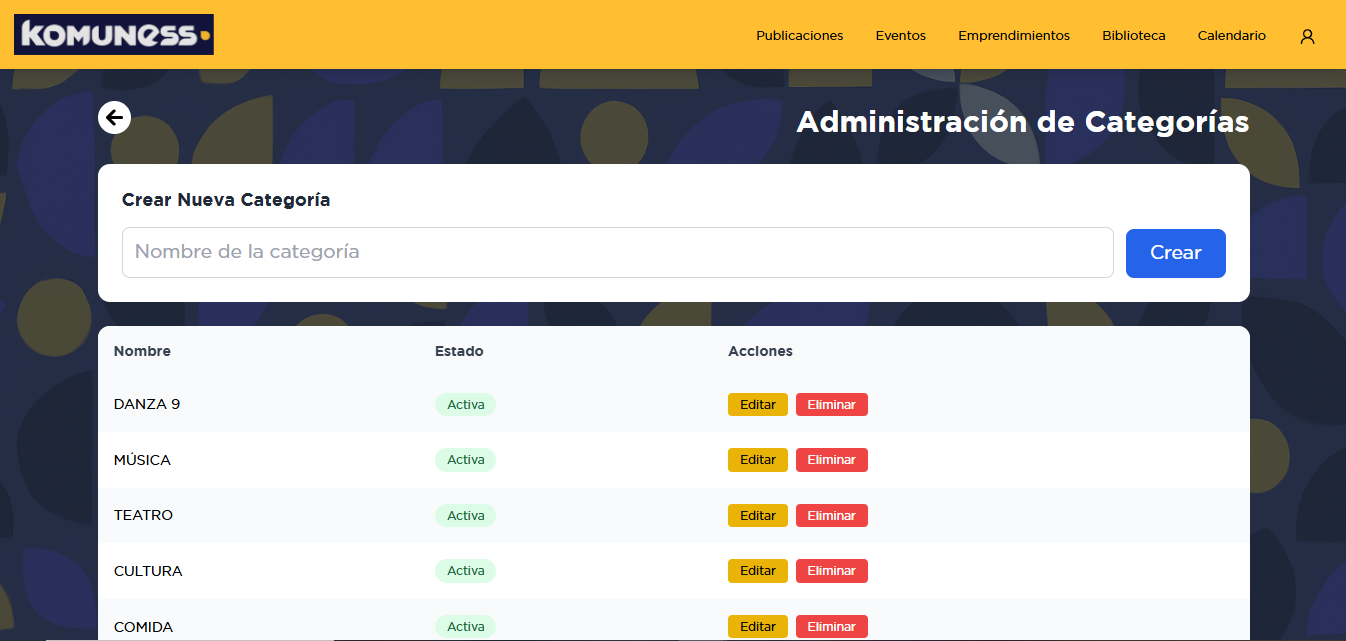
\includegraphics[width=0.9\textwidth]{project/images/imagen.PNG}
  \caption{Panel de administración de categorías - Vista principal con listado de categorías y opciones CRUD}
  \label{fig:categorias-admin}
\end{figure}

Características principales:
\begin{itemize}
  \item Vista tabular con opciones de crear, editar y eliminar.
  \item Formulario modal con campos: nombre, descripción y tipo.
  \item Validaciones en tiempo real para evitar duplicados.
  \item Confirmaciones de eliminación para prevenir pérdidas accidentales.
\end{itemize}

Características de usabilidad:
\begin{itemize}
  \item Botones con iconografía universal.
  \item Feedback visual inmediato (notificaciones de éxito/error).
  \item Búsqueda y filtrado en tiempo real.
  \item Diseño adaptativo para móviles y escritorio.
\end{itemize}

\subsection{Interfaz de Selección de Categorías (Usuario)}

La Figura~\ref{fig:categorias-selector} muestra cómo se integran las categorías en formularios de creación de publicaciones.

\begin{figure}[H]
  \centering
  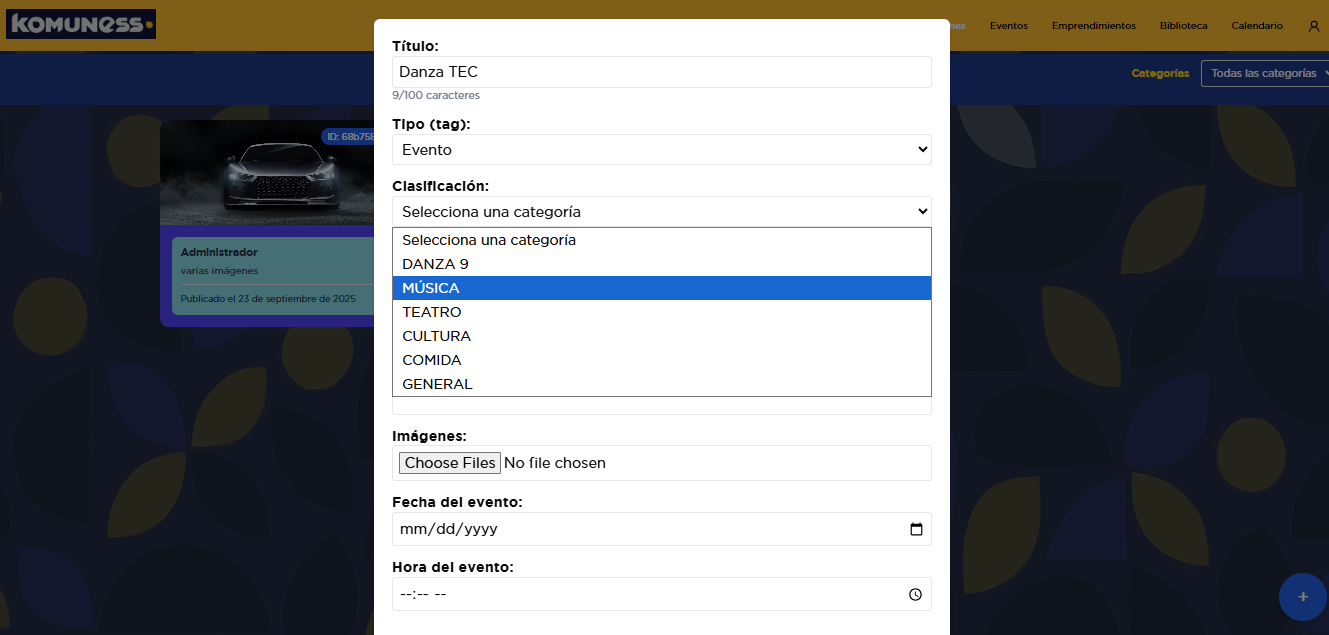
\includegraphics[width=0.8\textwidth]{project/images/imagen2.png}
  \caption{Selector de categorías integrado en formulario de creación de publicaciones}
  \label{fig:categorias-selector}
\end{figure}

\begin{itemize}
  \item Dropdown intuitivo integrado en formularios.
  \item Vista previa de la categoría seleccionada.
\end{itemize}

\begin{itemize}
  \item Badges visuales con categorías disponibles.
  \item Filtrado dinámico del contenido.
  \item Combinación de filtros (categoría + texto + autor).
  \item Indicador visual de filtros activos con opción de limpiar.
\end{itemize}

\begin{figure}[H]
  \centering
  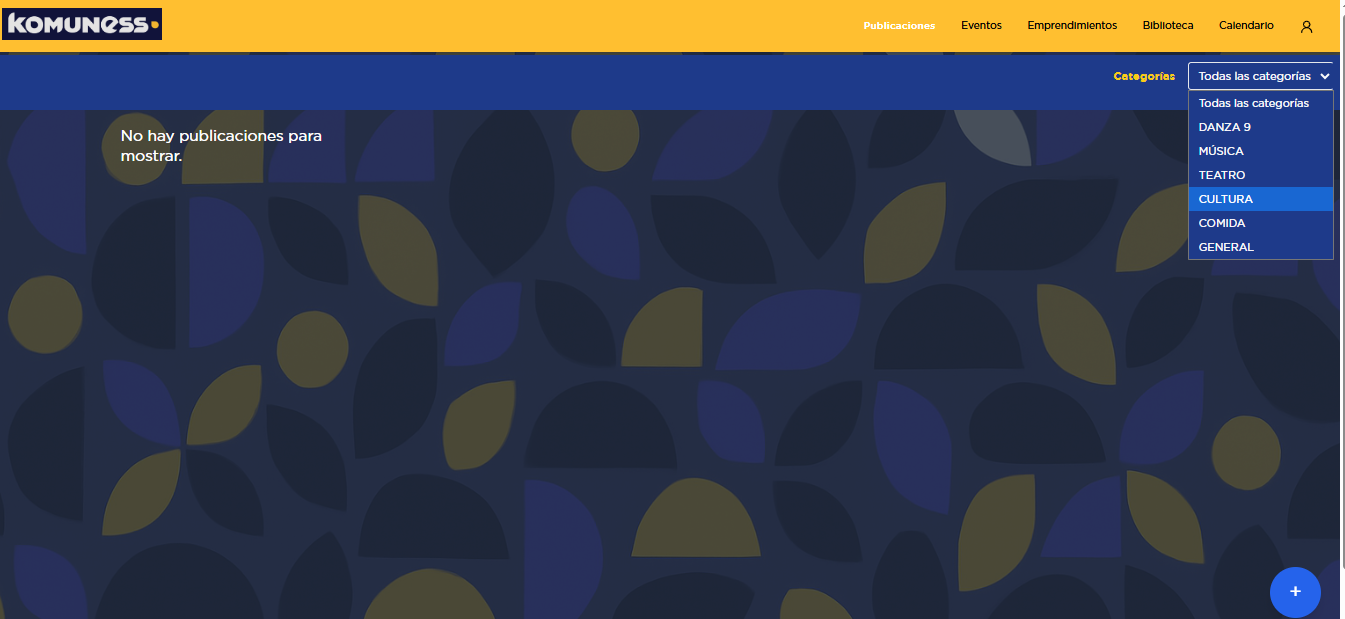
\includegraphics[width=0.9\textwidth]{project/images/imagen3.png}
  \caption{Sistema de filtros por categorías con badges visuales y filtrado dinámico}
  \label{fig:categorias-filtros}
\end{figure}

Principios de accesibilidad aplicados:
\begin{itemize}
  \item Contraste de colores (WCAG 2.1 AA).
  \item Texto alternativo en imágenes.
  \item Navegación completa por teclado.
  \item Tamaños de fuente escalables.
\end{itemize}

\section{Prototipos de la funcionalidad de Calendario Interactivo}

El calendario interactivo organiza eventos comunitarios, mejorando la participación en actividades.

\subsection{Vista Principal del Calendario}

La Figura~\ref{fig:calendario-vista} muestra la vista mensual del calendario.

\begin{figure}[H]
  \centering
  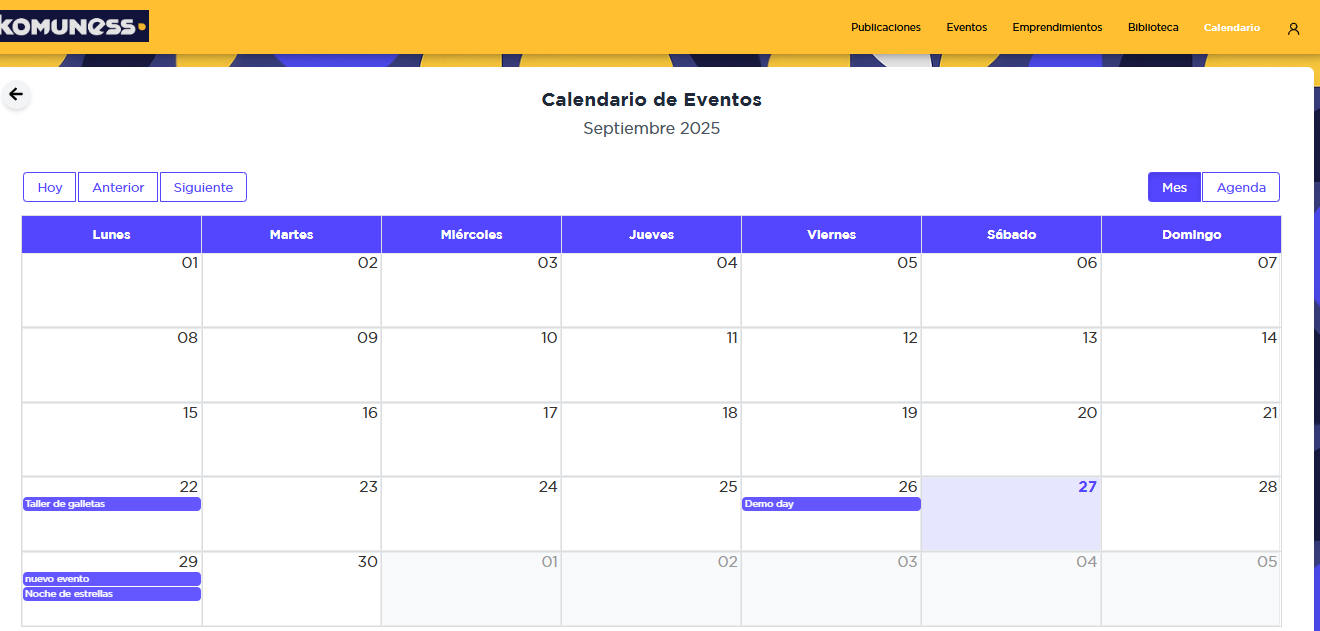
\includegraphics[width=0.9\textwidth]{project/images/imagen4.png}
  \caption{Vista principal del calendario interactivo con eventos marcados por fechas}
  \label{fig:calendario-vista}
\end{figure}

Características:
\begin{itemize}
  \item Layout en grid con eventos en fechas específicas.
  \item Navegación por meses (anterior/siguiente).
  \item Indicadores visuales por tipo de evento.
  \item Hover con información básica del evento.
\end{itemize}

\subsection{Vista de agenda}

La Figura~\ref{fig:calendario-detalle} muestra el panel lateral  eventos proximo.

\begin{figure}[H]
  \centering
  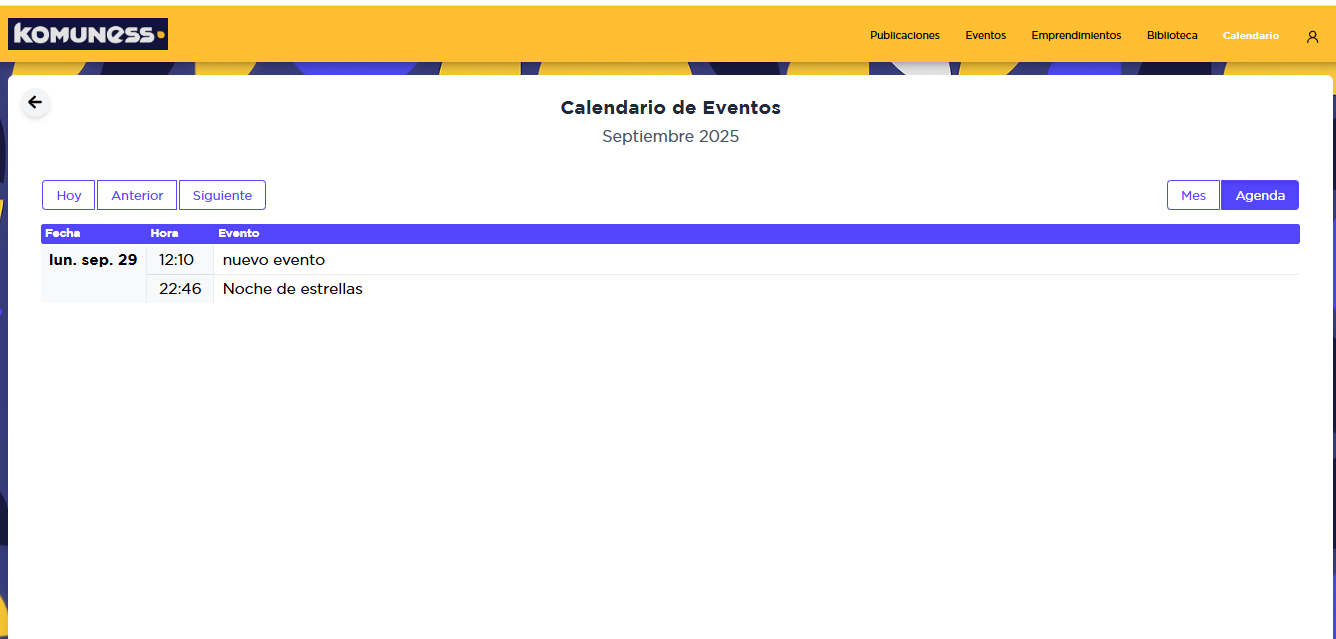
\includegraphics[width=0.8\textwidth]{project/images/imagen5.PNG}
  \caption{Panel de agenda de eventos con campos especificos}
  \label{fig:calendario-detalle}
\end{figure}

\begin{itemize}
  \item Información: fecha, hora, evento.

\end{itemize}

\subsection{Creación de Eventos}

La Figura~\ref{fig:calendario-crear} muestra el formulario de creación de eventos.

\begin{figure}[H]
  \centering
  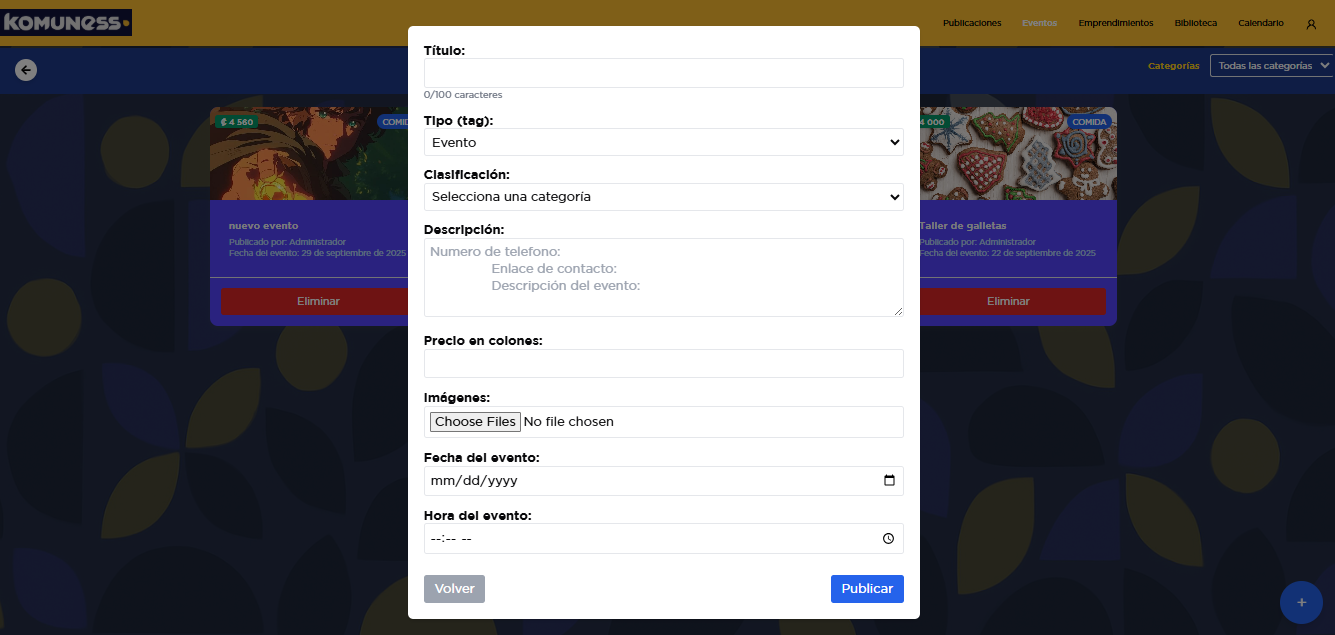
\includegraphics[width=0.85\textwidth]{project/images/imagen6.PNG}
  \caption{Formulario especializado para creación de eventos}
  \label{fig:calendario-crear}
\end{figure}

\begin{itemize}
  \item Campos: Titulo, Tag, Clasificación,Descripcion, Imagenes, Fecha del evento, Hora del evento.
  \item Validaciones: no permitir eventos sin información completa.
  \item Preview en tiempo real.
\end{itemize}

\subsection{Biblioteca Digital Optimizada}

Figura~\ref{fig:biblioteca} muestra la nueva vista con sistema de carpetas y filtros.

\begin{figure}[H]
  \centering
  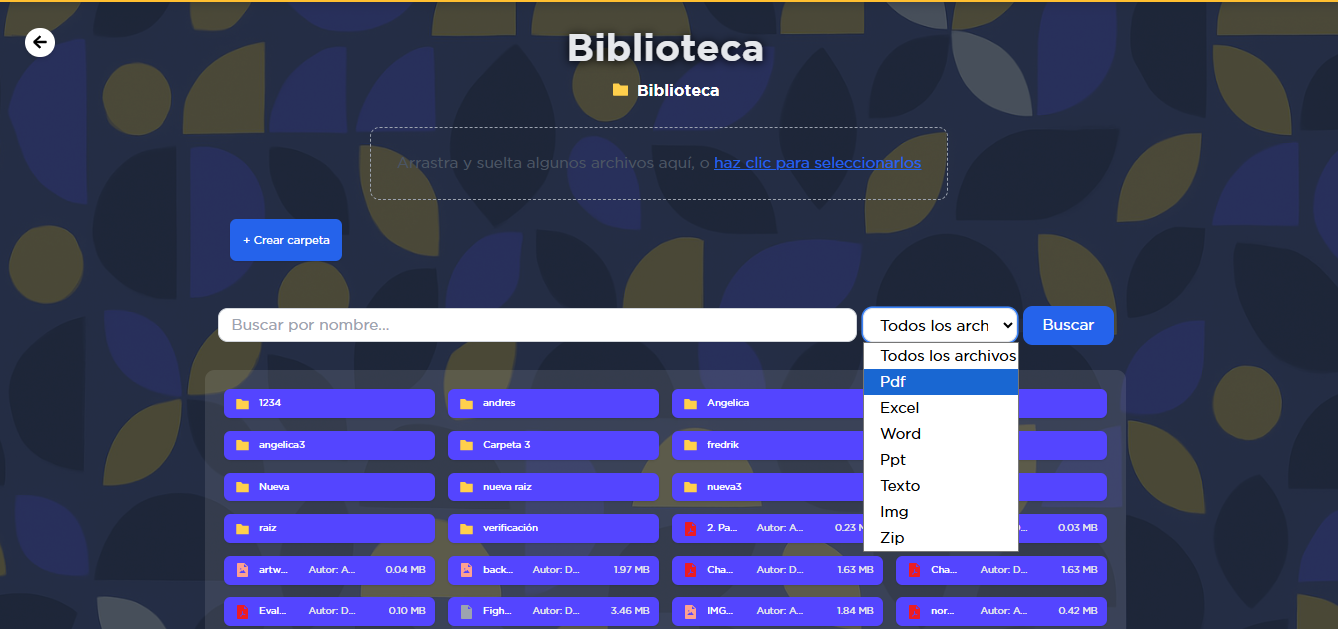
\includegraphics[width=0.9\textwidth]{project/images/imagen7.png}
  \caption{Vista de biblioteca digital optimizada con carpetas y filtros de búsqueda}
  \label{fig:biblioteca}
\end{figure}

\subsection{Diseño Responsive}

La Figura~\ref{fig:responsive} muestra la adaptación a distintos dispositivos.

\begin{figure}[H]
  \centering
  % Opción 1: ancho fijo en centímetros
  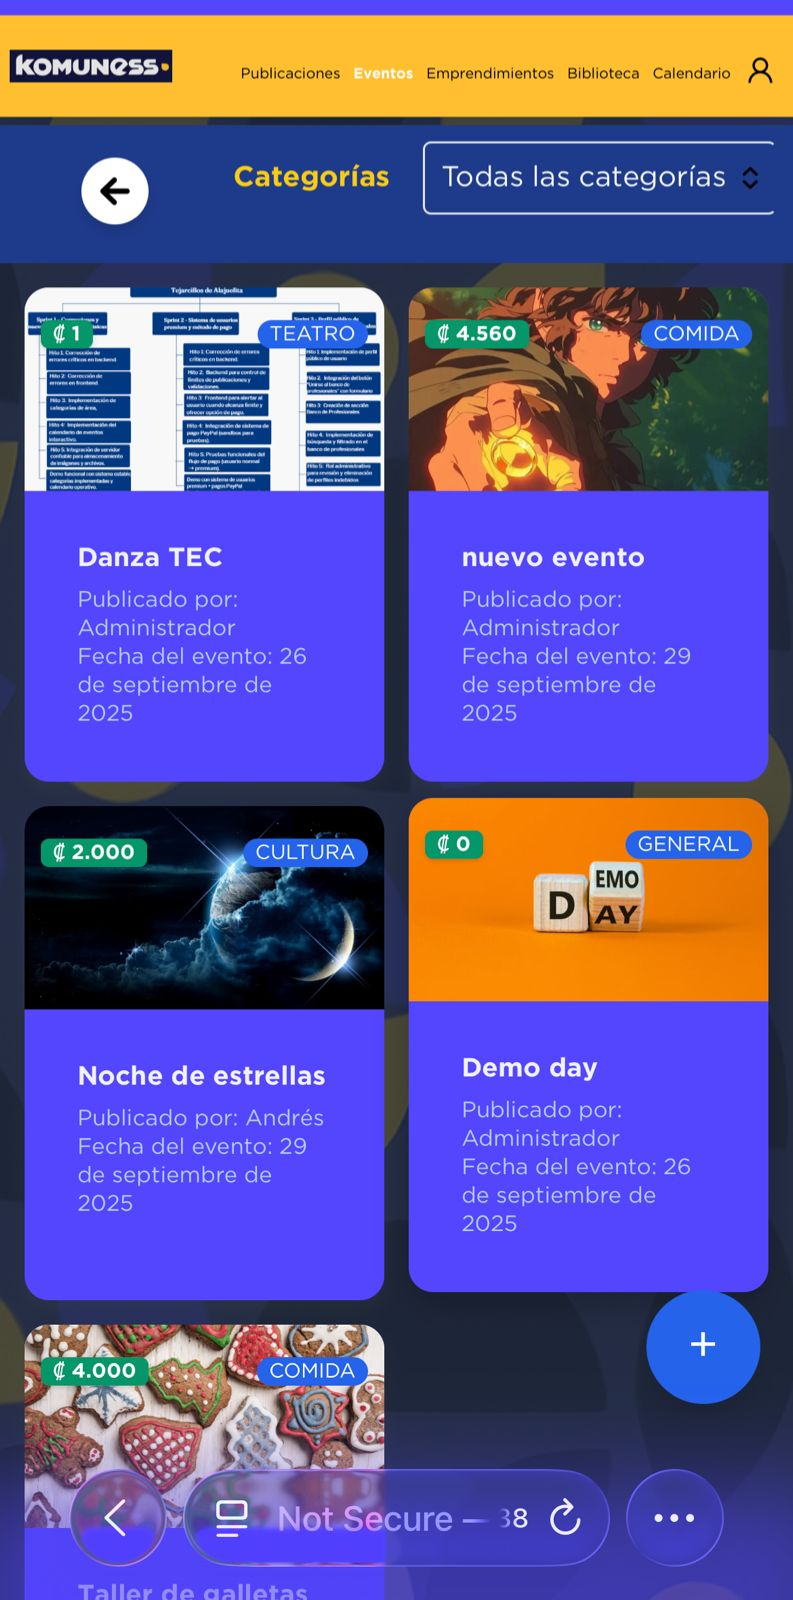
\includegraphics[width=4cm,keepaspectratio]{project/images/imagen8.jpg}
  
  % Opción 2: usar scale (reduce al 20% del tamaño original)
  %\includegraphics[scale=0.2]{project/images/responsive}

  % Opción 3: limitar ancho y alto para que nunca sea inmensa
  %\includegraphics[width=6cm,height=10cm,keepaspectratio]{project/images/responsive}

  \caption{Vista responsive en dispositivos móviles}
  \label{fig:responsive}
\end{figure}


\subsection{Características de Diseño y Usabilidad}

\begin{itemize}
  \item Transiciones suaves entre vistas.
  \item Estados de carga y vacíos informativos.
  \item Iconografía clara y culturalmente relevante.
  \item Touch targets grandes para móviles.
  \item Mensajes de error claros y confirmaciones visuales.
\end{itemize}
